\label{par:contrib1:convergence}
À présent que les stabilités des deux méthodes ImEx ont été comparées au \textit{splitting} d'opérateur, 
il est naturel de poursuivre par une expérience numérique pour évaluer la convergence de chaque méthode et 
d'évaluer la pertinence des méthodes ImEx face au \textit{splitting}.\par
\textbf{Présentation de l'expérience: }
    L'expérience est réalisée sur l'équation de Nagumo 1D à partir d'une solution initiale correspondant au profil de l'onde propagative de l'équation (voir \ref{par:analyser_operateurs_nagumo}).
    A la simulation a lieu sur le domaine spatial $[-20,+20]$ entre $t=0$ et $t=3$.
    La grille spatiale est divisée en $2^{13}$ cellules ce qui équivaut à un pas d'espace $\Delta t \approx 4.8 \, 10^{-3}$.
    Des conditions de Neumann homogènes et une vitesse de propagation adaptées permettent de maintenir le front d'onde au centre du domaine et 
    de négliger les effets de bords afin de comparer à la solution analytique exacte d'onde propagative.\par
\textbf{Résultats: }
    Les résultats de l'expérience sont présentés en \ref{fig:imex_vs_splitting}. Il apparaît que si le schéma de splitting et l'ImEx222 ont des performances similaires, la méthode ImEx232
    présente une constante de convergence plus faible. De fait on voit que sur un maillage classique (non-adapté en espace), les méthodes ImEx peuvent apporter une cohérence globale qui mène a 
    une meilleure précision. Dans la section suivante, l'expérience est réitérée sur un maillage adapté par multi-résolution adaptative pour étudier si l'adaptation en espace 
    interagit différemment avec les méthodes ImEx et la méthode de splitting.
    \begin{figure}[hb!]
        \centering
        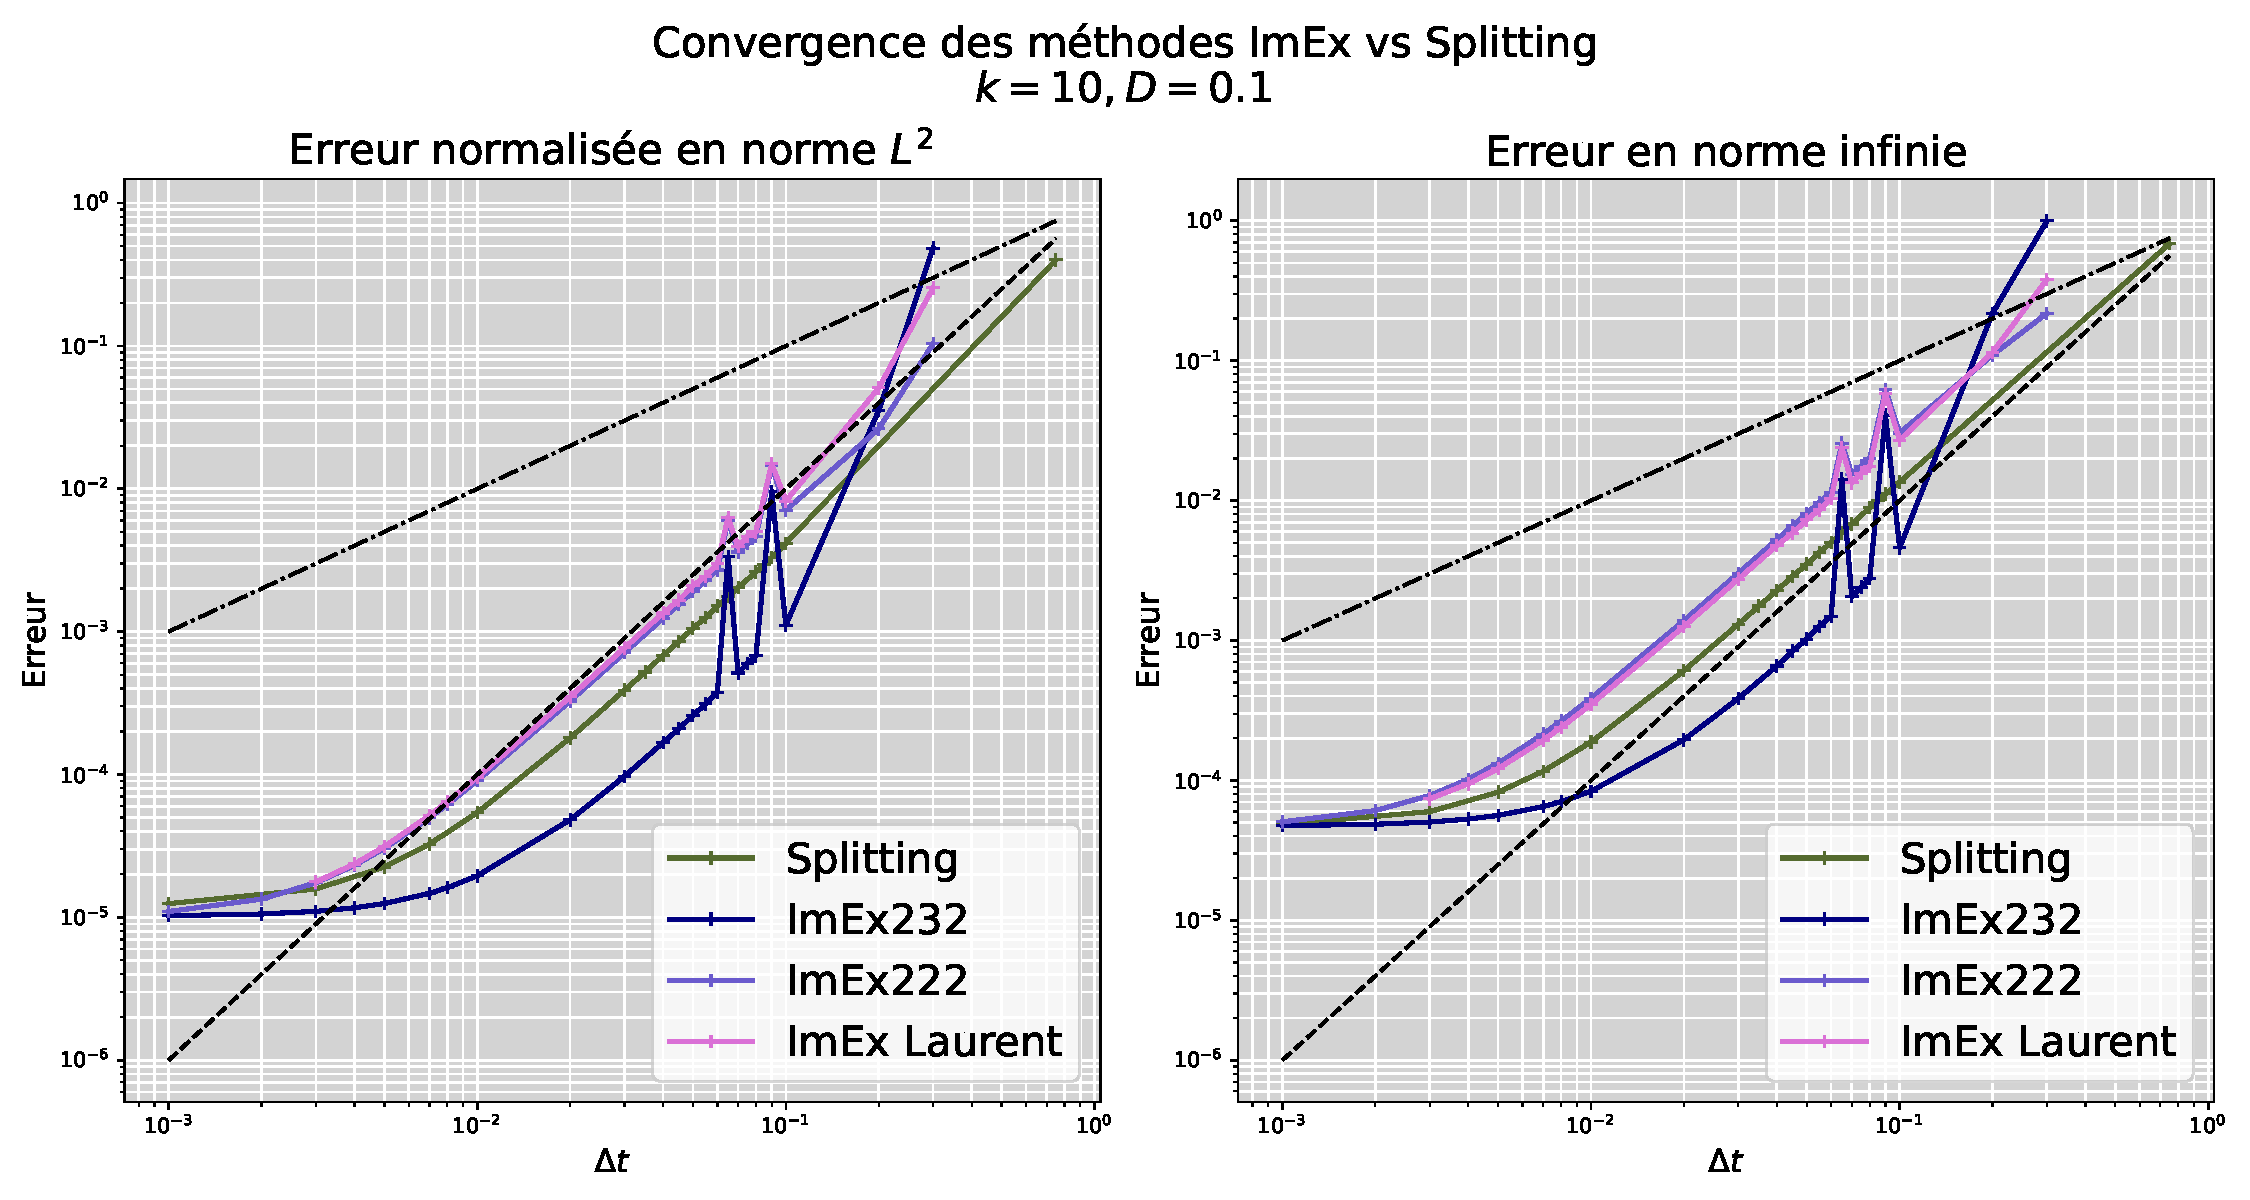
\includegraphics[width=\linewidth]{media/4_travail/2_nagumo/convergence/ImEx_vs_splitting_k10_D0.1.pdf}
    \caption{Comparaison de la convergence du schéma de splitting avec celle des méthodes ImEx222 et ImEx232
    sur l'équation de Nagumo avec $D=0.1$ et $k=10$}
    \label{fig:imex_vs_splitting}
    \end{figure}
\newpage
\subsection{Mise en lumière expérimentale de couplages entre la méthode en temps et l'adaptation spatiale}
\label{par:couplagetempsadaptation}
\textbf{Objectifs et contexte de l'étude: }
L'objectif est d'observer d'éventuelles interactions entre la méthode de découplage des opérateurs (ImEx/splitting) et l'adaptation en espace par multi-résolution adaptative.
Pour ce faire la comparaison entre ImEx222, ImEx2332 et splitting a été refaite (fig \ref{fig:couplage-MRA-temps}) en adaptant spatialement chaque schéma par MRA.
Si des différences par rapport à l'étude précédente (fig. \ref{fig:imex_vs_splitting}) apparaissent, ils résultent nécessairement de couplages entre la méthode d'intégration en temps
et l'adaptation spatiale.\par
\begin{figure}[htbp!]
    \centering
    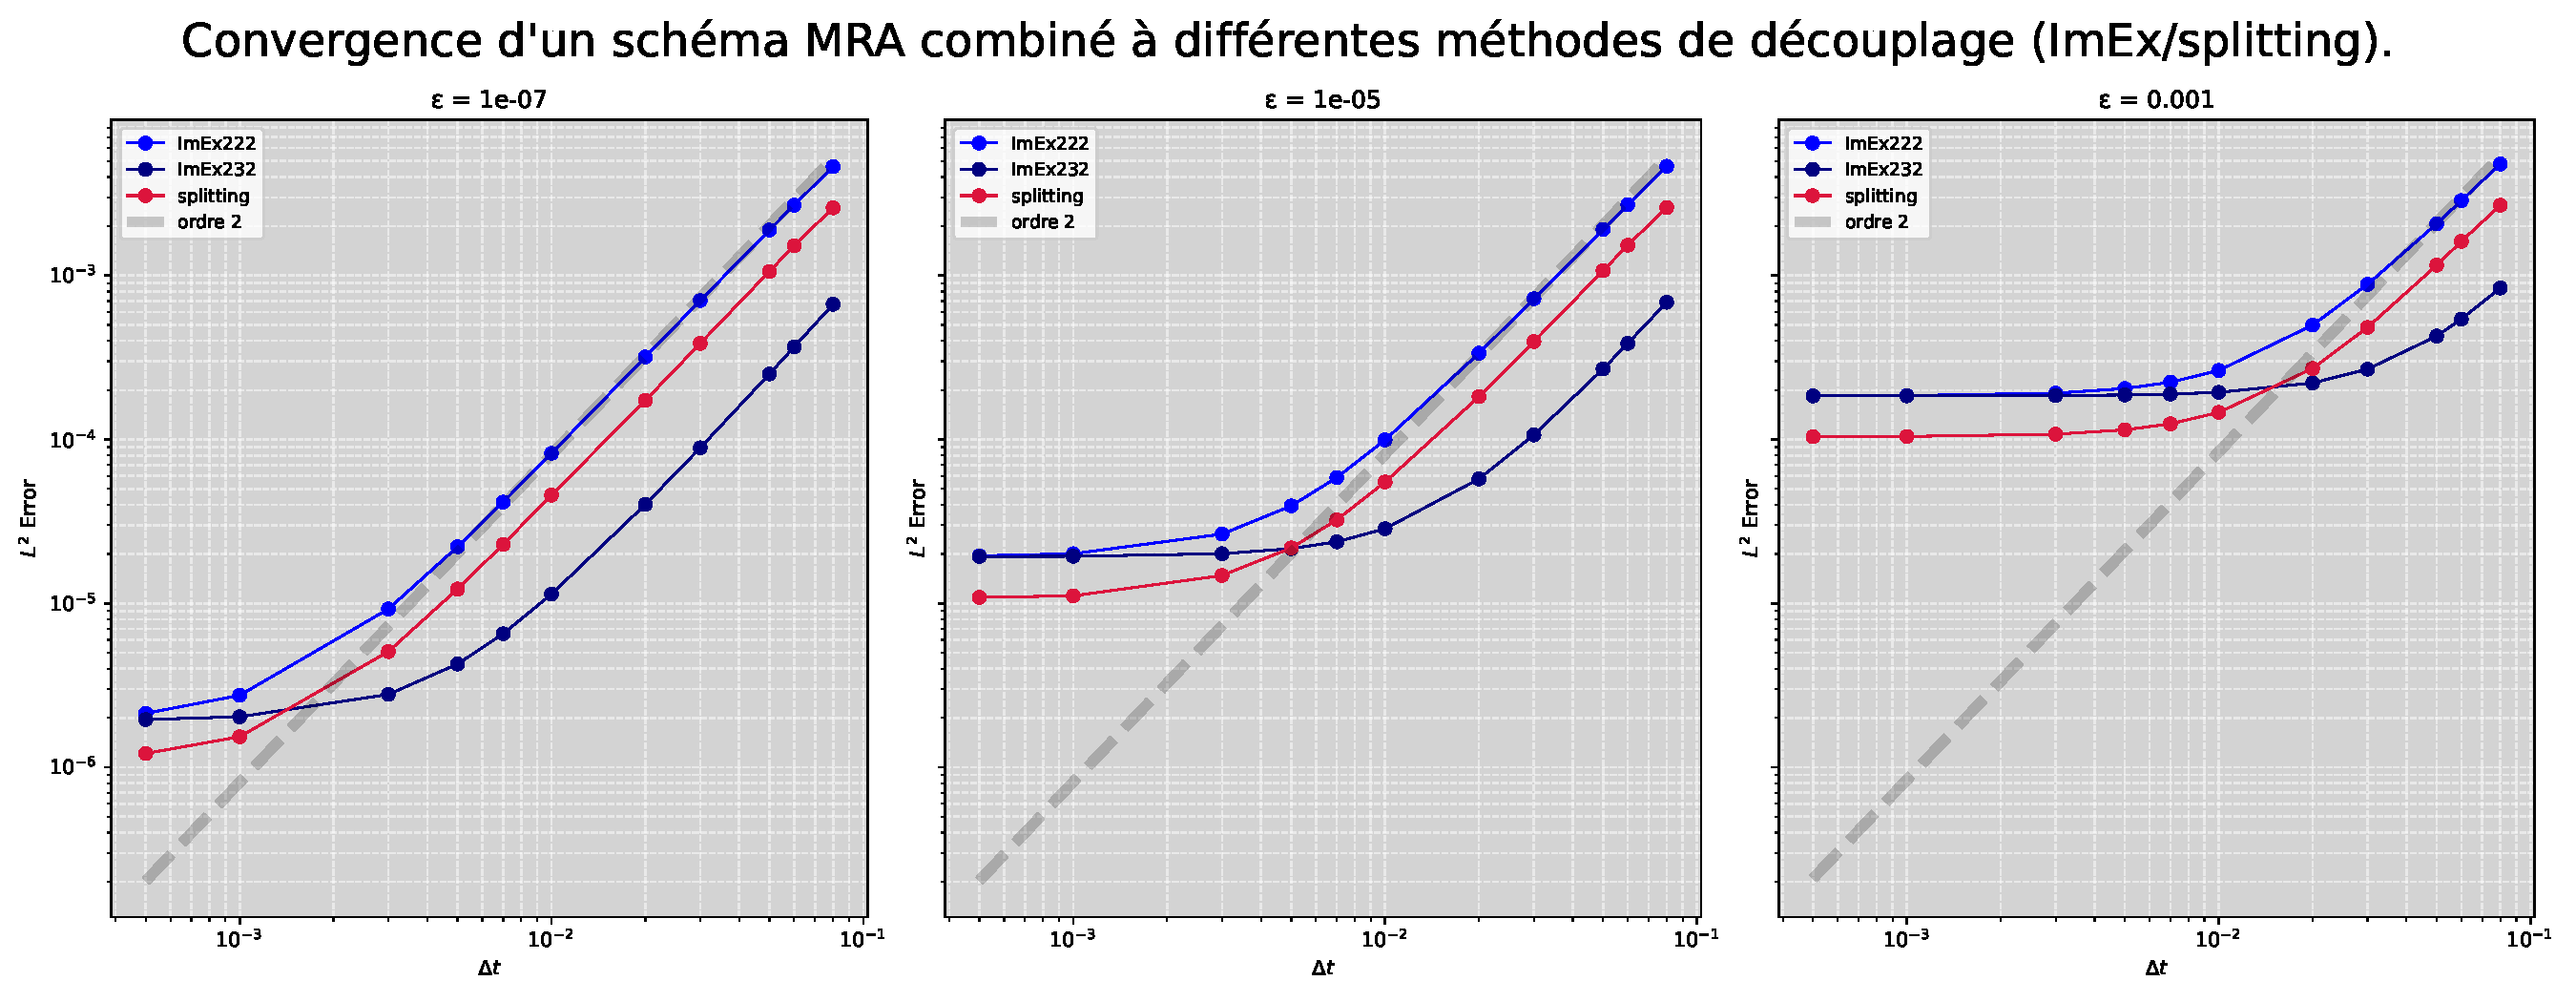
\includegraphics[width=\linewidth]{media/4_travail/2_nagumo/couplage/couplage_MRA_temps.pdf}
    \caption{Convergence des schémas ImEx et de splitting, adaptés en espace par MRA, sur l'équation de Nagumo pour $k=10$, $D=0.1$.
    Les flux sont évalués au niveau courant (\textit{cf.} \ref{par:contrib_2}), la prédiction/reconstruction est assurée par un prédicteur à trois points et l'erreur est comparé à une solution convergé en temps.}
    \label{fig:couplage-MRA-temps}
\end{figure}
\textbf{Analyse des résultats:} pour les grands pas de temps, la convergence est similaire au cas non-adapté (fig. \ref{fig:imex_vs_splitting}). En particulier la méthode
ImEx232 exhibe toujours une constante de convergence plus faible que le splitting. 
En revanche, lorsque l'erreur sature les méthodes ImEx offrent systématiquement des performances moins bonnes que le splitting.
La solution est comparée à une méthode quasi-exacte en temps, la convergence s'infléchie donc lorsque les erreurs de liée à la MRA sont de l'ordre des erreurs en temps.
Il semble donc que l'erreur plateau soit composée d'une erreur de compression (commune aux trois méthodes) et d'une erreur de couplage entre l'adaptation spatiale
et le schéma. Plus précisément il semble que l'interaction adaptation-schéma soit plus néfaste pour les méthodes ImEx que pour le splitting.\\
% \textbf{Limites de l'étude:} ces résultats expérimentaux peuvent être impactés par de nombreux paramètres numériques. Par exemple,
% il n'est pas garantis que les résultats soient les mêmes pour un prédicteur à 5 points au lieu de 3.